\chapter{Rush Hour Intervention Human Subject Experiment}
\label{apx:rushintervention}
We discuss details about the Rush Hour human subject study and the findings. The following sections present the evidence on which we based the design choices for the Rush Hour planning task. The sections are cross-referenced throughout the main content.

\section{Rush Hour Human Subject Study: Pilot Experiment}
\label{ap:pilot}
Before the study was actually administered to our recruited subjects, a pilot study was conducted with nine graduate students to assess whether they would be able to solve the puzzles within a reasonable amount of time. The pilot study participants solved their assigned puzzles within 5-10 minutes. The pilot study participants were also interviewed informally to get their perception of the puzzle difficulty. The participants commented that the puzzles were ``\textit{challenging}'' and ``\textit{forced me to think}''. The same puzzles used in the pilot were used in the actual study.\\

\section{Demography Survey Findings}
\label{ap:demographics}
Majority of the participants (39) were below the age of 20, while 38 subjects were between the age 20-25. Maximum age was 41 years. 70 of the 117 participants were male. When asked if they liked puzzle solving tasks, 78\% of the participants either agreed or strongly agreed with the statement. Specifically to the Rush Hour game 79\% of the participants liked or strongly liked Rush Hour. The most common reason as to why the participants liked puzzle solving tasks was that puzzle solving stimulates critical thinking skills. 30\% of the participants usually did a puzzle solving task once a month, while 21\% of the participants solved a puzzle once a week. When asked about strategies the participants used to solve difficult puzzles, 79\% of the group said that they kept trying until the puzzle was eventually solved, while 12\% of the participants said that they would ask for help. 

Given a new puzzle that they have not seen before, if they get stuck while solving the puzzle, 26\% said that they would not like any outside help. 47\% of the participants said that they would like a suggestion/tip that would get them past the current situation. 15\% said that they would like a warning, which indicated that their current approach would lead to a dead-end. 8\% of the participants said that they would like a warning and an explanation to help them prevent getting stuck in the future.  The most common medium for solving puzzles was using their mobile devices (42\%). 31\% of the participants used the personal computers/laptops to solve puzzles. 19\% of the participants solved puzzles using physical means (e.g., puzzle books, newspapers and physical puzzles such as Rubik's  cubes).\\

\section{User Solutions Grouped by Length}
\label{ap:lengroups}
For each puzzle, we sorted the solutions by the number of moves (in the complete solution) in the ascending order and split them into three groups (fast, medium, slow). We ensured that the three groups for each puzzle contained approximately equal number of users. Table \ref{tab:solvergroups} summarizes the findings. There were 46 users in the fast group, 42 in the medium and 48 in the slow group. Mean refers to the mean number of moves in a solution produced by users who solved a specific puzzle. Forbidden moves refers to the number of times, the users who solved a specific puzzle moved the forbidden vehicle.

\begin{table}[ptb]
\begin{tabular}{|l|l|l|l|l|l|l|}
\hline
\multicolumn{1}{|c|}{\multirow{2}{*}{PID}} &
  \multicolumn{2}{c|}{Fast (46)} &
  \multicolumn{2}{c|}{Medium (42)} &
  \multicolumn{2}{c|}{Slow (48)} \\ \cline{2-7} 
\multicolumn{1}{|c|}{} &
  \multicolumn{1}{c|}{Mean} &
  \multicolumn{1}{c|}{\begin{tabular}[c]{@{}c@{}}Forbidden\\ Moves\end{tabular}} &
  \multicolumn{1}{c|}{Mean} &
  \multicolumn{1}{c|}{\begin{tabular}[c]{@{}c@{}}Forbidden\\ Moves\end{tabular}} &
  \multicolumn{1}{c|}{Mean} &
  \multicolumn{1}{c|}{\begin{tabular}[c]{@{}c@{}}Forbidden\\ Moves\end{tabular}} \\ \hline
P1  & 25.5 & 0  & 41.7  & 0  & 64.7  & 0  \\ 
P2  & 74.7 & 4  & 137.7 & 16 & 277   & 28 \\ 
P3  & 26.5 & 8  & 36.2  & 9  & 43.7  & 6  \\ 
P4  & 25.2 & 1  & 32    & 4  & 76    & 28 \\ 
P5  & 18.3 & 3  & 26    & 2  & 44.75 & 13 \\ 
P6  & 22   & 0  & 24.5  & 0  & 39.6  & 0  \\ 
P7  & 38.5 & 5  & 53.3  & 16 & 120   & 37 \\ 
P8  & 9    & 0  & 9     & 0  & 10    & 0  \\ 
P9  & 27.8 & 8  & 48.6  & 12 & 99    & 28 \\ 
P10 & 50.3 & 11 & 66    & 14 & 127.3 & 46 \\ \hline
\end{tabular}
\caption{Plans produced by human users grouped by the mean number of moves and the number of forbidden moves}
\label{tab:solvergroups}
\end{table}

\section{Solution Length Distribution}
\label{ap:distribution}
\begin{figure}[tpb]
  \centering
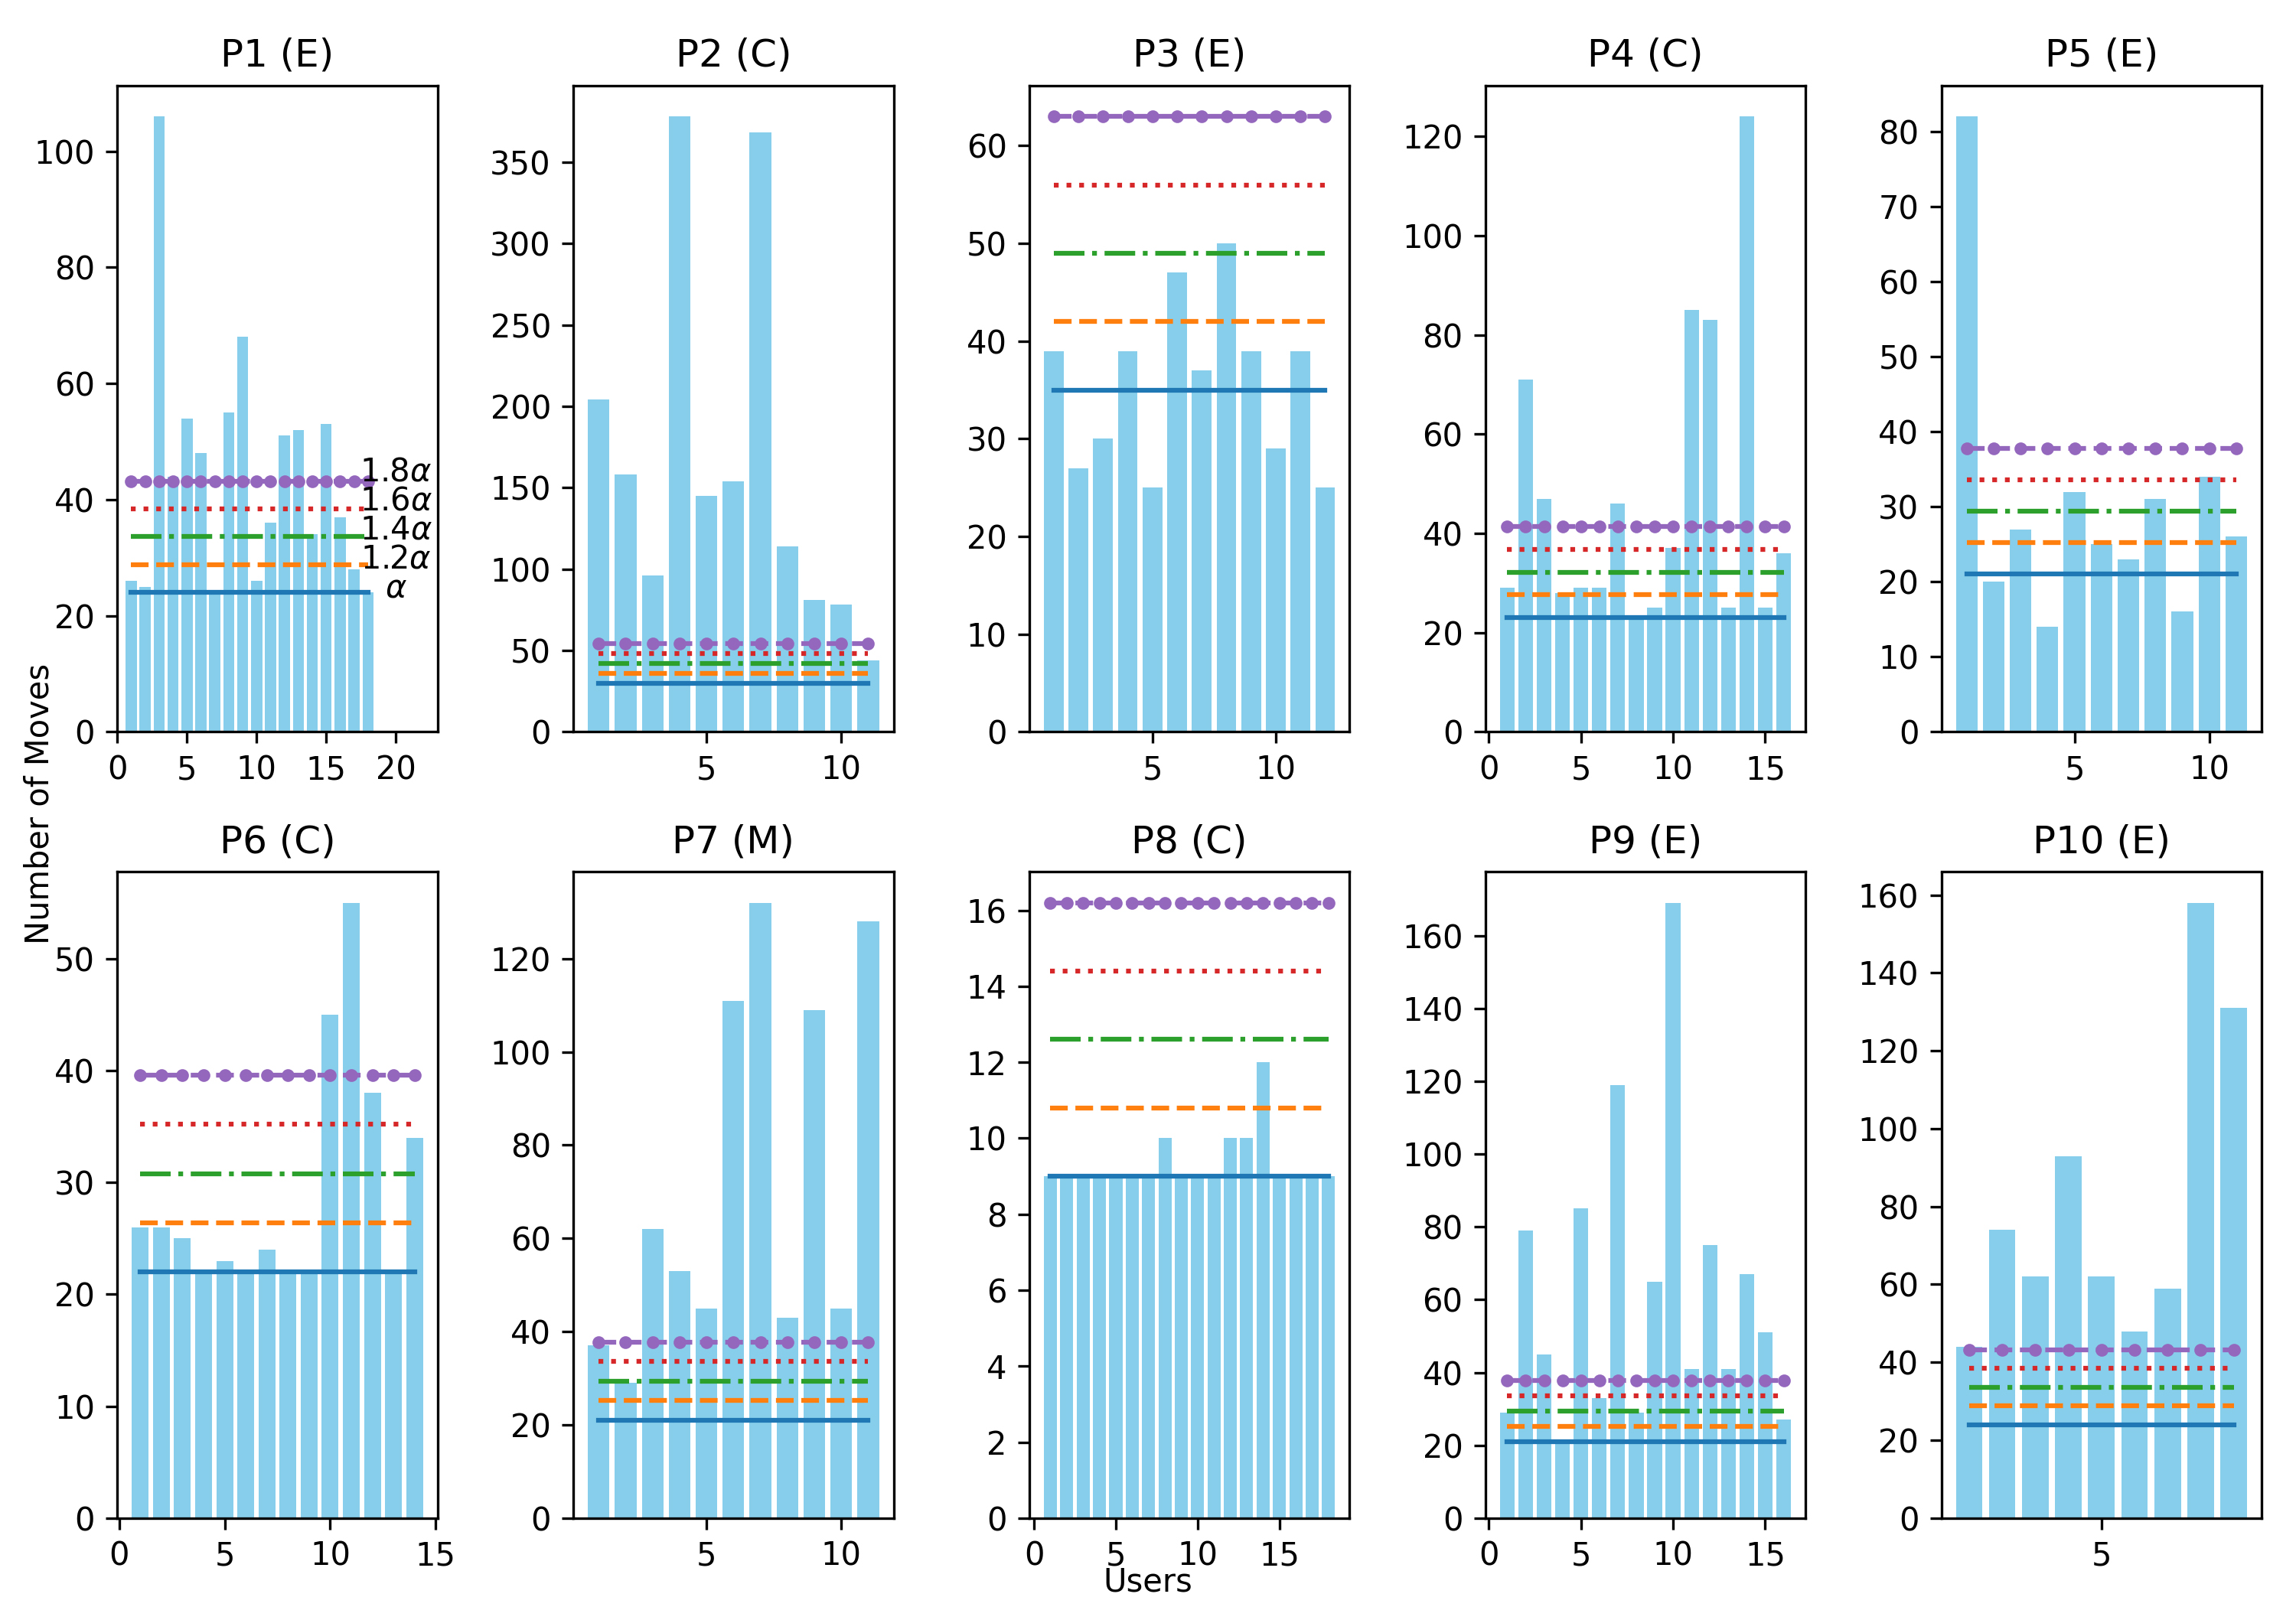
\includegraphics[width=\columnwidth]{img/figure7.jpg}
  \caption{Number of moves in the users' solution compared to the optimal number of moves $\alpha$, 1.2$\alpha$, 1.4$\alpha$, 1.6$\alpha$, 1.8$\alpha$ for puzzles P1 through P10}
  \label{fig:difficulty}
\end{figure}

Figure~\ref{fig:difficulty} illustrates how the number of moves in users' solutions compare to a set of threshold values derived from the optimal solution for each Rush Hour planning task. We define the threshold set $\theta$ as: given the optimal number of moves  $\alpha$ for a puzzle, $\theta=\lbrace \alpha, 1.2\alpha, 1.4\alpha, 1.6\alpha, 1.8\alpha\rbrace$. The letter in parenthesis indicates the puzzle group (see Figure~\ref{fig:ui}(B) for the three puzzle types) of each puzzle.

It can be seen that human solvers' solutions to P8 were very close to the optimal solution in the number of moves. Human solvers' found it very difficult to find a solution closer to the optimal number of moves for P2.
Users who attempted P3 and P5 found solutions shorter than the safe, optimal. Shorter solutions for these two puzzles all required the user to move the forbidden vehicles.